% !TeX root = ../main.tex

\chapter{Methodology and implementation}\label{chapter:Methodology and implementation}

In order to find the CVSS3 score of a set of bugs found through compositional symbolic execution, we needed to go through a set of very rigorous steps, that had to be sequential since all of them relied on the one that came just before it.

\section{Research phase}

With our motivation in mind, and a specific goal set, we set out to research all the components that would be needed. All successes and failures will be noted, so that futre work on this area may use this work to avoid some pitfalls.

It is also worth noting that we will touch on all the main technologies involved in the entirety of the process, though not going to specifics when the involvement of the technology does not require much user intervention, such as in the case of LLVM for instance.

\subsection{Understanding LLVM}

Analysing source code can prove difficult, specially programs that need to be compiled, such being the case of our thesis, where we will be working with C and C++ source code. The reason why it could prove difficult is that the relationships between functions, and classes -- in the case of C++ -- can be lost when for example, cleansing the data for text mining. It could also be possible to analyze binaries, but this would prove difficult since it would only allow us to see the results of the compilation, and again could lead to losing some accuracy and important data during compilation.

Symbolic execution tools (e.g KLEE, or MACKE) require the input to be bitcode, specifically compiled with LLVM. The bitcode is an intermediate point where it can still be altered with, to some extent (since the source code is completely tokenized), while keeping its structure.

The LLVM compiler infrastructure project (formerly Low Level Virtual Machine) is a "collection of modular and reusable compiler and toolchain technologies" used to develop compiler front ends and back ends.

LLVM is written in C++ and is designed for compile-time, link-time, run-time, and "idle-time" optimization of programs written in arbitrary programming languages. Originally implemented for C and C++, the language-agnostic design of LLVM has since spawned a wide variety of front ends: languages with compilers that use LLVM include ActionScript, Ada, C Common Lisp, Crystal, D, Delphi, Fortran, OpenGL Shading Language, Halide, Haskell, Java bytecode, Julia, Lua, Objective-C, Pony, Python, R, Ruby, Rust, CUDA, Scala, Swift, and Xojo.

The LLVM project started in 2000 at the University of Illinois at Urbana–Champaign, under the direction of Vikram Adve and Chris Lattner. LLVM was originally developed as a research infrastructure to investigate dynamic compilation techniques for static and dynamic programming languages.

The name LLVM was originally an initialism for Low Level Virtual Machine, but this became increasingly less apt as LLVM became an "umbrella project" that included a variety of other compiler and low-level tool technologies, so the project abandoned the initialism. Now, LLVM is a brand that applies to the LLVM umbrella project, the LLVM intermediate representation (IR), the LLVM debugger, the LLVM C++ Standard Library (with full support of C++11 and C++14), etc. LLVM is administered by the LLVM Foundation. \parencite{llvm}

\subsection{Getting to know KLEE}

The program now known as KLEE\parencite{klee} stemed from EXE \parencite{exeBook} which was a program that allowed for symbolic execution, or code that can generate its own test cases as they mention. To better exemplify how EXE worked, which is still the core of KLEE, we have the following code:

\begin{figure}[!htb]
	\caption{C program analyzed by EXE}
	\centering
	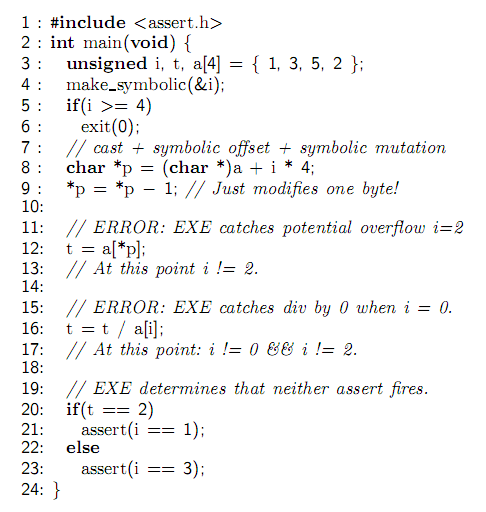
\includegraphics[width=0.6\textwidth]{code_example_exe}
\end{figure}

It shows how different errors may come to be, and some of them could lead to an exploitable vulnerability. This code also has several branches that can be taken, which are shown in the following figure:

\begin{figure}[!htb]
	\caption{EXE symbolic execution}
	\centering
	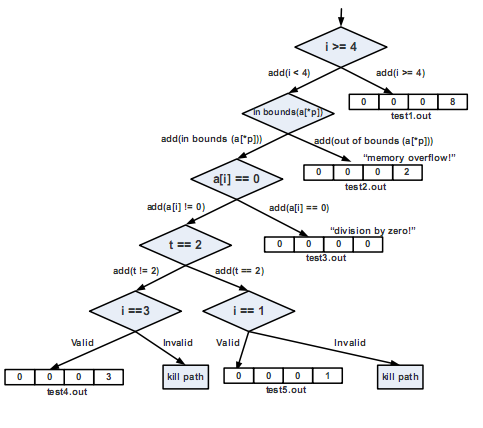
\includegraphics[width=0.6\textwidth]{code_example_graph_exe}
\end{figure}

And as shown, EXE had as one of its limitations, that it could only deal with branches where numeric values where used, as it happens in the example showcased in Figure 2.2 . KLEE has built upon this work, and now is what their developers call 

\enquote{\texttt{A hybrid
		between an operating system for symbolic processes and
		an interpreter. Each symbolic process has a register file,
		stack, heap, program counter, and path condition}} \parencite{klee}
	

 All programs must be compiled to the LLVM  assembly language. KLEE directly interprets this instruction set, and maps instructions to constraints without approximation, since it uses bit-level accuracy.\parencite{klee}
 
 KLEE requires no modification of the source file, only that it has been compiled with LLVM, and run the bitcode directly through KLEE. What KLEE will do, is the same thing that EXE previously did, which is add symbolic parts in the code -- when possible --, but introducing all the aforementioned benefits.
 
 KLEE's results are quite thorough, though for our research we only need the main JSON file that it generates with: functions where vulnerabilities have been found, and their respective JSON file that contains all the details of how this vulnerability came to be / was found.
 
 The problem that KLEE has is that generates test cases by starting at the entry point of the program (forward symbolic execution), resulting in insufficient code coverage, which will leave many vulnerabilities unfound. Though there is a tool that allows for compositional symbolic execution, which alows for a much better code coverage, thus granting us a much higher chance of finding vulnerabilities across a given program. Its name is MACKE (Compositional Analysis of Low-Level
 Vulnerabilities with Symbolic Execution). \parencite{ognawala}
 

\subsection{Compositional symbolic execution through MACKE}

The program MACKE, was designed to solve the issue that forward symbolic execution had, by using a three-step approach. Its developer describes the tool's approach in the following manner: 

\enquote{\texttt{MACKE is based on the modular interactions inferred
		by static code analysis, which is combined with symbolic execution
		and directed inter-procedural path exploration. This
		provides an advantage in terms of statement coverage and
		ability to uncover more vulnerabilities.}}\parencite{ognawala}
	
How MACKE goes about doing this is by splitting what would normally just be a forward symbolic execution of a program, like KLEE would -- from which MACKE originated -- into three steps.

\enquote{\texttt{Firstly,
		MACKE performs symbolic execution on the individual components
		of a program, in isolation. This has the advantage
		of higher code coverage and ability to uncover many lowlevel
		vulnerabilities in all program components. Secondly,
		MACKE uses results of the first step to reason about (and,
		therefore, reduce the number of) reported vulnerabilities
		from a compositional perspective, i.e. by finding feasible
		inter-procedural paths for those vulnerabilities to be exploited.
		Thirdly, MACKE assigns severity scores to reported
		vulnerabilities by considering several characteristic features
		and provides the result in an interactive visual format.}}\parencite{ognawala}
	
What this provides is a much higher chance of finding vulnerabilities in the code, because of a much more fine grain code coverage.

The usage of MACKE is quite similar to that of KLEE; the program must be compiled with LLVM, so that a bitcode file is available, which is the used as the input of MACKE. There is no need to modify the source code in order for it to work.

MACKE's results are very robust, and showcases the three-step execution it goes through. The main resulting file is "klee.json" which includes the function names of only those where vulnerabilities where found. 
It shows whether the vulnerability was found in phase 1, which means if the vulnerability was found when each of the components of the program were isolated and executed. If it shows phase 2, it means that the vulnerability was found at a lower level, and found by using the results of phase 1. 

\subsection{Call graphs}

By compiling our programs with LLVM we are able to get a bitcode file, which includes all interactions between the program's components (i.e functions, interfaces..). This file will also allow us to generate a call graph of such interactions.

A call graph is a flow graph, that showcases in a form of a set of nodes connected to each other, how all functions from a given program interact between each other, in other words, their relationships. Callgrahs are directed graphs, which entails that all nodes will have edges (f,g) indicating that functiong f calls function g. For instance if a node X has an edge with (X,X) it means that it is calling itself, making it a recursive function.

The purpose of call graphs is to display in a human readable way, how a program interacts internally, which can allow programmers to quickly pinpoint where a bottleneck, or security flaw may be. It also serves as a starting point when analyzing the design of an application. If there are disconnected nodes, or redundant nodes, it is quickly visible at first glance, so that proper action can be taken.

\begin{figure}[!htb]
	\caption{AutoTrace 0.31.1}
	\centering
	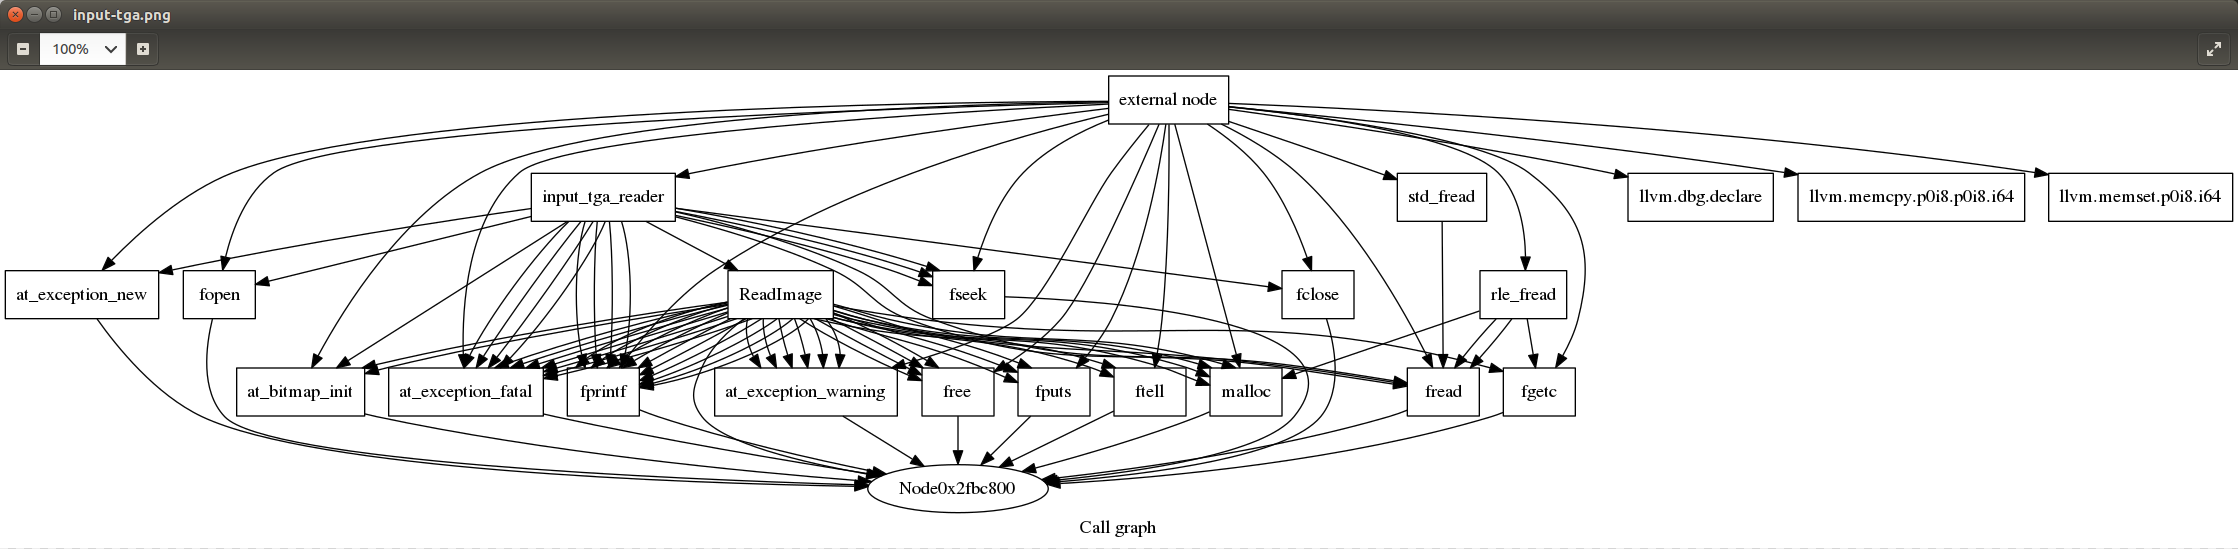
\includegraphics[width=1.0\textwidth]{callgraph}
\end{figure}

There are two types of callgraphs. The first one is dynamic, which displays how the relationships during runntime look. This callgraph can vary depending on what commands were given to a program upon its start-up. The second one is static, and as the name implies, it never changes. A static call graph shows every single call, regardless of whether it may or not be called during the program's runtime.\parencite{callgraphs}

In this case we extract a static callgraph, as seen in Figute 2.3 it is clearly visible how a static callgraph overaproximates the amount of calls of a given function to another. Using "ReadImage" as an example, it calls "fprintf" several times in this callgraph. The code looks as follows:

\begin{lstlisting}
static at_bitmap_type ReadImage (FILE *fp,
struct tga_header *hdr,
at_exception_type * exp);
at_bitmap_type
input_tga_reader (at_string filename,
at_input_opts_type * opts,
at_msg_func msg_func, 
at_address msg_data)
{
	FILE *fp;
	struct tga_header hdr;
	
	at_bitmap_type image = at_bitmap_init(0, 0, 0, 1);
	at_exception_type exp = at_exception_new(msg_func, msg_data);
	
	fp = fopen (filename, "rb");
	if (!fp)
	{
		LOG1 ("TGA: can't open \"%s\"\n", filename);
		at_exception_fatal(&exp, "Cannot open input tga file");
	}
	
	/* Check the footer. */
	if (fseek (fp, 0L - (sizeof (tga_footer)), SEEK_END)
	|| fread (&tga_footer, sizeof (tga_footer), 1, fp) != 1)
	{
		LOG1 ("TGA: Cannot read footer from \"%s\"\n", filename);
		at_exception_fatal(&exp, "TGA: Cannot read footer");
		goto cleanup;
	}
	
	/* Check the signature. */
	
	if (fseek (fp, 0, SEEK_SET) ||
	fread (&hdr, sizeof (hdr), 1, fp) != 1)
	{
		LOG1 ("TGA: Cannot read header from \"%s\"\n", filename);
		at_exception_fatal(&exp, "TGA: Cannot read header");
		goto cleanup;
	}
	
	/* Skip the image ID field. */
	if (hdr.idLength && fseek (fp, hdr.idLength, SEEK_CUR))
	{
		LOG1 ("TGA: Cannot skip ID field in \"%s\"\n", filename);
		at_exception_fatal(&exp, "TGA: Cannot skip ID field");
		goto cleanup;
	}
	
	image = ReadImage (fp, &hdr, &exp);
	cleanup:  
	fclose (fp);
	return image;
}
\end{lstlisting}

It is not so clear to see, but the C library function int fprintf(FILE *stream, const char *format, ...) sends formatted output to a stream. It is being used on every line where a logentry is made. It clearly shows how only one of these log entries will be made per function call, and not all of them, so it is redundant, yet that is how static call graphs over aproximate calls (f,g).

The advantage of having a static call graph is that we can see every single path possible, and the redundancies -- function X with repeated outbound edges(X,Y) or inbound edges(Y,X) -- can be removed.

What is important about the call graphs is that they can be analyzed by using graph logic.

\subsection{Directed graphs and Node Attributes}

Graph theory \parencite{graphs} is the mathematical area that focuses on the analysis of the structure of graphs. A graph can be directed or undirected, the former having vertices that do not depict a source and a target, but only a relation between the two, while the latter does have a source and target, and as the name implies, having a direction, as it was explained in 2.1.4 .

As it also has been explained, we are dealing with static callgraphs which are always directed graphs. Therefore, we set out to explore the different attributes that could be extracted. To this end, we explored graph attributes for classification from \parencite{graphClassification} which we found concise and well documented, as well as using generic formulas from \parencite{graphs}. 

We will be exploring, and explaining to detail what the considered graph attributes were, and which ones worked for our thesis.

\subsubsection{Node degree}

Every node has a degree which is the amount of its neighboring edges. So if a node has 2 outgoing edges and 3 incoming, its degree is 5. This works both for directed and undirected graphs.

\begin{figure}[!htb]
	\caption{Node degree}
	\centering
	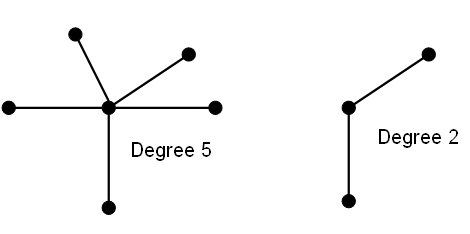
\includegraphics[width=0.5\textwidth]{node_degree}
\end{figure}

We thought of this value as extremely important, because it shows how intertwined a function is. What we mean by this, is that if it is very centric, the probability of a vulnerability spreading from this point or falling into the vulnerability is likely to be higher. Needless to say, this attribute was chosen to be implemented in our framework.

\subsubsection{Clustering coefficient}

The definition of this attribute is :

\enquote{\texttt{For node $u$, the clustering coefficient $c(u)$ represents the likelihood that any two neighbors of $u$ are connected.}}\parencite{graphClassification}

\begin{figure}[!htb]
	\caption{Clustering coefficient}
	\centering
	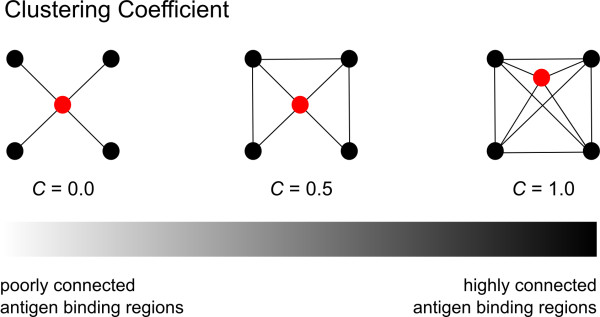
\includegraphics[width=0.5\textwidth]{clustering_coefficient}
\end{figure}

In other words, the amount of triangles of node $u$ , divided by the number of triples a node $u$ has.

We also found this attribute to be relevant to our analysis, since it also shows the relations of a node to its surrounding nodes, but also how much it relies on other functions, as well as how much other functions rely on it.

\subsubsection{Effective eccentricity}

The definition of this attribute is :

\enquote{\texttt{For effective eccentricity we take the
		maximum length of the shortest path from u, so that
		u can reach at least 90 percent of nodes in the graph.
		Effectiveness is a more robust measure if we take noise
		into consideration. The average effective eccentricity
		is the average of effective eccentricities of all nodes in the graph.
}}\parencite{graphClassification}

This attribute would not be of good use in our case, since the likelihood of a node reaching 90\% of the graph in a directed graph is very low, and this attribute would most of the time be extremely low, unless it was an interface, which would only be one node. Needless to say, this was discarded and completely disregarded.

\subsubsection{Path length}

The definition of this attribute is :

\enquote{\texttt{Average path length (closeness centrality): The
		closeness centrality of a node u is defined as the reciprocal of the averaged total path length between node
		u and every other node that is reachable from node
		u.		
}}\parencite{graphClassification}

In other words, if we have the root be the node, and average the distance to its children nodes (every single one, regardless of their level), this will give us the closeness centrality of that given node.

This attribute complements the degree and the clustering coefficient nicely, and adds another angle of analysis. This was selected as another attribute to be used in our framework.

It is worth noting that the description we have given, and used only applies to directed graphs, where sources and targets are available, thus explicitly showing the relationships between nodes (e.g parent, child, etc...)

\section{Node attributes found through MACKE}

Getting outside of the realm of graph attributes, and into the results found by MACKE, we were able to get two very valuable node attributes, that we could use for every single function.

\subsubsection{Vulnerabilities found by Macke}

This node attribute depicts how many vulnerabilities MACKE was able to find, like shown in Figure 3.6 . For every vulnerability found, a counter would go up for the function affected. Therefore, if a function had 3 vulnerabilities found, that is the value this node attribute would hold for that specific function.

\subsubsection{Macke bug chain length}

This node attribute tells us how long a chain of calls was before the vulnerable function was called. To do this, we checked the phase in which each function was called. If a bug was found during phase two, we checked the caller and the callee of each function, until we reached the vulnerability. If a chain was, for instance, 5 functions long, that would be the value represented by this node attribute.

\subsection{Exploring CVSS base scores, and their meaning}

In our introduction to this thesis, we introduced CVSS -- which we will be naming CVSS3, to explicitly specify that we use version 3.0 throughout this project -- and its importance towards achieving our goal of assessing vulnerabilities as objectively as possible. We also introduced the base scores, what they mean, and how they impact the assessment. Now we will describe in detail what each base score can have as its value, and what each one means.

All of the following information has been taken from \parencite{cvss3} as our source, to stay true and consistent.

\subsubsection{Attack Vector (AV)}

\begin{itemize}
	\item Network (N) - A vulnerability exploitable with network access means the vulnerable component is bound to the network stack and the attacker's path is through OSI layer 3 (the network layer). Such a vulnerability is often termed "remotely exploitable” and can be thought of as an attack being exploitable one or more network hops away.
	\item Adjacent (A) - A vulnerability exploitable with adjacent network access means the vulnerable component is bound to the network stack, however the attack is limited to the same shared physical (e.g. Bluetooth, IEEE 802.11), or logical (e.g. local IP subnet) network, and cannot be performed across an OSI layer 3 boundary (e.g. a router).
	\item Local (L) - A vulnerability exploitable with local access means that the vulnerable component is not bound to the network stack, and the attacker’s path is via read/write/execute capabilities. In some cases, the attacker may be logged in locally in order to exploit the vulnerability, otherwise, she may rely on User Interaction to execute a malicious file.
	\item Physical (P) - A vulnerability exploitable with physical access requires the attacker to physically touch or manipulate the vulnerable component. Physical interaction may be brief or persistent.
\end{itemize}

To sumarize this base score, we can say that the more distance there can be between the attacker and the system, the more vulnerable the system is.

\subsubsection{Attack Complexity (AC)}

\begin{itemize}
	\item Low (L) - Specialized access conditions or extenuating circumstances do not exist. An attacker can expect repeatable success against the vulnerable component.
	\item High (H) - A successful attack depends on conditions beyond the attacker's control. That is, a successful attack cannot be accomplished at will, but requires the attacker to invest in some measurable amount of effort in preparation or execution against the vulnerable component before a successful attack can be expected. For example, a successful attack may require the attacker: to perform target-specific reconnaissance; to prepare the target environment to improve exploit reliability; or to inject herself into the logical network path between the target and the resource requested by the victim in order to read and/or modify network communications (e.g. a man in the middle attack).
\end{itemize}

To sumarize this base score, we can say that the more distance there can be between the attacker and the system, the more vulnerable the system is.

\subsubsection{Privileges Required (PR)}

\begin{itemize}
	\item None (N) - The attacker is unauthorized prior to attack, and therefore does not require any access to settings or files to carry out an attack.
	\item Low (L) - The attacker is authorized with (i.e. requires) privileges that provide basic user capabilities that could normally affect only settings and files owned by a user. Alternatively, an attacker with Low privileges may have the ability to cause an impact only to non-sensitive resources.
	\item High (H) - The attacker is authorized with (i.e. requires) privileges that provide significant (e.g. administrative) control over the vulnerable component that could affect component-wide settings and files.
\end{itemize}

The more requirements the attacker requires, the less severe the vulnearbility is. When it is regarded as "High" the CVSS3 score drops quite drastically, because it means that there are measures in place to keep attackers at bay.

\subsubsection{Privileges Required (PR)}

\begin{itemize}
	\item None (N) - The attacker is unauthorized prior to attack, and therefore does not require any access to settings or files to carry out an attack.
	\item Low (L) - The attacker is authorized with (i.e. requires) privileges that provide basic user capabilities that could normally affect only settings and files owned by a user. Alternatively, an attacker with Low privileges may have the ability to cause an impact only to non-sensitive resources.
	\item High (H) - The attacker is authorized with (i.e. requires) privileges that provide significant (e.g. administrative) control over the vulnerable component that could affect component-wide settings and files.
\end{itemize}

The more requirements the attacker requires, the less severe the vulnearbility is. When it is regarded as "High" the CVSS3 score drops quite drastically, because it means that there are measures in place to keep attackers at bay.

\subsubsection{User Interaction (UI)}

\begin{itemize}
	\item None (N) -The vulnerable system can be exploited without any interaction from any user.
	\item Required (R) - Successful exploitation of this vulnerability requires a user to take some action before the vulnerability can be exploited. 
\end{itemize}

If the attacker requires a user of the system to interact with, for example a malisious script, the severity would drop quite drastically.

\subsubsection{Scope (S)}

\begin{itemize}
	\item Unchanged (U) - An exploited vulnerability can only affect resources managed by the same authority. In this case the vulnerable component and the impacted component are the same.
	\item Changed (C) - An exploited vulnerability can affect resources beyond the authorization privileges intended by the vulnerable component. In this case the vulnerable component and the impacted component are different. 
\end{itemize}

This base score refers to the state of the system when attacked, and how many privileges the attacker will have after the attack in comparisson to its prior  unaffected state.

\subsubsection{Confidentiality (C)}

\begin{itemize}
	\item None (N) - There is no loss of confidentiality within the impacted component.
	\item Low (L) - There is some loss of confidentiality. Access to some restricted information is obtained, but the attacker does not have control over what information is obtained, or the amount or kind of loss is constrained. The information disclosure does not cause a direct, serious loss to the impacted component. 
	\item High (H) - There is total loss of confidentiality, resulting in all resources within the impacted component being divulged to the attacker. Alternatively, access to only some restricted information is obtained, but the disclosed information presents a direct, serious impact.
\end{itemize}

This base score refers to the amount of data accessible to the attacker after the attack. If this base score is high, the vulnerability will be affected severely.

\subsubsection{Integrity (I)}

\begin{itemize}
	\item None (N) - There is no loss of integrity within the impacted component.
	\item Low (L) - Modification of data is possible, but the attacker does not have control over the consequence of a modification, or the amount of modification is constrained. The data modification does not have a direct, serious impact on the impacted component.
	\item High (H) - There is a total loss of integrity, or a complete loss of protection. For example, the attacker is able to modify any/all files protected by the impacted component. Alternatively, only some files can be modified, but malicious modification would present a direct, serious consequence to the impacted component.
\end{itemize}

The more data is modifiable after the attack, the more severe the vulnerability is. This most of the time is linked to confidentiality since it handles privileges.

\subsubsection{Availability (A)}

\begin{itemize}
	\item None (N) - There is no impact to availability within the impacted component.
	\item Low (L) - There is reduced performance or interruptions in resource availability. Even if repeated exploitation of the vulnerability is possible, the attacker does not have the ability to completely deny service to legitimate users. The resources in the impacted component are either partially available all of the time, or fully available only some of the time, but overall there is no direct, serious consequence to the impacted component.
	\item High (H) - There is total loss of availability, resulting in the attacker being able to fully deny access to resources in the impacted component; this loss is either sustained (while the attacker continues to deliver the attack) or persistent (the condition persists even after the attack has completed). Alternatively, the attacker has the ability to deny some availability, but the loss of availability presents a direct, serious consequence to the impacted component (e.g., the attacker cannot disrupt existing connections, but can prevent new connections; the attacker can repeatedly exploit a vulnerability that, in each instance of a successful attack, leaks a only small amount of memory, but after repeated exploitation causes a service to become completely unavailable).
\end{itemize}

\section{Implementation phase}

Now that we have a clearer picture of all the pieces of the puzzle, we need to make it all come together. In order for us to be able to do this, we had to make a very specific plan, and do all of the steps shown in this chapter sequentally, since each one depended on to one that came right before it.

\subsection{Finding a reliable Vulnerabilities Database and suitable programs to analyze}

The first thing we had to do was find a database of vulnerabilities, that was not only reliable, but also provided precise CVSS3 scores -- or at least as detailed, and up-to-date as possible -- so that we could use this information as a starting point.

The main idea behind getting vulnerabilities that have already been found and assessed manually, is that we could try to find the same vulnerability by different means, in this case, through composite symbolic execution using MACKE. By having done that, means that we would have a bitcode file, which could be then used to get a callgraph of the program. Here is where the CVSS3 scores come into play.

The CVSS3 scores from the database must be very accurate, reliable and thorough, since they would be our basis of analysis when comparing against the call graph. The main idea is that through the analysis of the callgraph and the attributes mentioned in 2.1.5 we could generate an algorithm that could assess these scores as precisely as possible.

\subsubsection{Bugzilla database}
First we started by taking a look at Bugzilla\parencite{bugzilla}, since it is widely adapted in the industry and has a large developer base. They also can rate the severity of a bug -- though manually done -- which they call Severity as well, and describe as:

\enquote{\texttt{How severe the bug is, or whether it's an enhancement.}}\parencite{bugzilla}

It's worth noting that their use of the word "bug" is very broad in the Bugzilla project, and covers ultimately every type of vulnerability found. 

They also divide severity into three four categories depending on their impact which are as follows:

\begin{table}[!htb]
	\centering
	\caption{Bugzilla's Severity Categories}
\begin{tabular}{ |p{4cm}||p{9cm}|  }
	\hline
	Category & Description\\
	\hline
	Critical   & crashes, memory leaks and similar problems on code that is written in a common enough style to affect a significant fraction of users   \\
	Normal &   major loss of functionality \\
	Minor & minor loss of functionality, misspelled word, or other problem where an easy workaround exists \\
	Enhancement    & Request for enhancement \\
	\hline
\end{tabular}
\end{table}

Also, they do not use the severity of a given vulnerability only, they also use the Priority which they describe as:

\enquote{\texttt{Engineers prioritize their bugs using this field.}}\parencite{bugzilla}

The description of Priority can be quite obscure, and hard to understand, since it is not described what it means, and could change from one user of Bugzilla to the next. By combining Severity and Priority they get their Importance attribute which is their final assessment of a vulnerability.

While their assessment of the Importance is good, and could work, it was of no use to us since it relied on a subjective part, which they call Priority. Furthermore, they do not use CVSS, neither 2.0 nor 3.0, therefore any Bugzilla database would be of no use. Therefore, we moved on to NVD.

\subsubsection{NVD - National Vulnerability Database}

By looking at gouvernmental vulnerability databases, we came across a USA based database, which not only is it up to date, but it also is funded by the government of said country. Their own description can be found bellow:\\

\enquote{\texttt{The NVD  is the U.S. government repository of standards based vulnerability management data represented using the Security Content Automation Protocol (SCAP). This data enables automation of vulnerability management, security\\ measurement, and compliance. The NVD includes databases of security checklist references, security related software flaws, misconfigurations, product names, and impact metrics.
\\
Originally created in 2000 (called Internet - Categorization of Attacks Toolkit or ICAT), the NVD has undergone multiple iterations and improvements and will continue to do so to deliver its services. The NVD is a product of the NIST Computer Security Division, Information Technology Laboratory and is sponsored by the Department of Homeland Security’s National Cyber Security Division.
\\
The NVD performs analysis on CVEs that have been published to the CVE Dictionary. NVD staff are tasked with analysis of CVEs by aggregating data points from the description, references supplied and any supplemental data that can be found publicly at the time. This analysis results in association impact metrics (Common Vulnerability Scoring System - CVSS), vulnerability types (Common \\Weakness Enumeration - CWE), and applicability statements (Common Platform Enumeration - CPE), as well as other pertinent metadata. The NVD does not actively perform vulnerability testing, relying on vendors, third party security researchers and vulnerability coordinators to provide information that is then used to assign these attributes. As additional information becomes available CVSS scores, CWEs, and applicability statements are subject to change. The NVD endeavors to re-analyze CVEs that have been amended as time and resources allow to ensure that the information offered is up to date.}}\parencite{nvd}
\\\\
This database completely aligns with our needs, as it provides extremely reliable content -- approved by the government of the USA, and backed up by the NIST (National Institute of Standards and Technology) -- and has up to date CVSS3 scores, as well as having a broad range of programming languages, including C/C++. 

\subsubsection{Getting vulnerabilities and their source code}

Once we settled on the database, we knew we had to find vulnerabilities that met the following criteria:

\begin{enumerate}
	\item Open source program
	\item C or C++ code
	\item Function where the vulnerability lies is documented
	\item CVSS3 scores available
\end{enumerate}

Knowing that we started going through the database, starting from the year CVSS3 started being used by NVD, which was 2016. After going through the entirety of the database, it was hard to find programs that met the aforementioned criteria, yet we did find them.

The programs found are:

\begin{itemize}
	\item BlueZ 5.42
	\item AutoTrace 0.31.1
	\item AutoTrace 0.31.1
	\item GraphicsMagic 1.3.25
	\item Icoutils 0.31.1
	\item ImageMagic 6.0.4-8
	\item Jasper 1.900.27
	\item Jasper 2.0.10
	\item Libarchive 3.2.1
	\item Libass 0.13.3
	\item Libmad 0.15.1
	\item Libplist 1.12
	\item Libdsndfile 1.0.28
	\item Libxml2 2.9.4
	\item Lrzip 0.631
	\item Openslp 2.0.0
	\item Potrace 1.12
	\item Rzip 2.1
	\item Tcpdump 4.9.0
	\item Tif Dirread
	\item Virglrenderer 0.5.0
	\item Ytnef 1.9.2
\end{itemize}

All of these programs met all of our requirements. We were able to find their source code, all of which were C and C++, and they all had extremely detailed CVSS3 scores.

\subsection{Running all programs through MACKE}

Now that we had the programs we could test if MACKE would be able to find the vulnerabilities noted in the NVD database.
What had to be done first is run all of the make files in order to get all the source code needed for our specific system, and then run LLVM over them.

We took advantage of a tool developed internally at TUM called "make+llvm"\parencite{thomasThesis} that does just that in one simple step, the only thing that is needed to be done is select the make file, and it takes care of the rest.

By the end of the make+llvm run, we are greeted with all of the bitcode files for all .c or .cpp files that were encountered in the program (and that were needed upon compilation). These files are crucial to our research because:

\begin{enumerate}
	\item We can generate a callgraph of the program / function
	\item We can run MACKE on them
\end{enumerate}

With all of the files we followed to run MACKE on exactly the bitcode generated for the specific .c where the vulnerability was found and documented in the NVD database.

\begin{figure}[!htb]
	\caption{MACKE vulnerabilities found for AutoTrace 0.31.1}
	\centering
	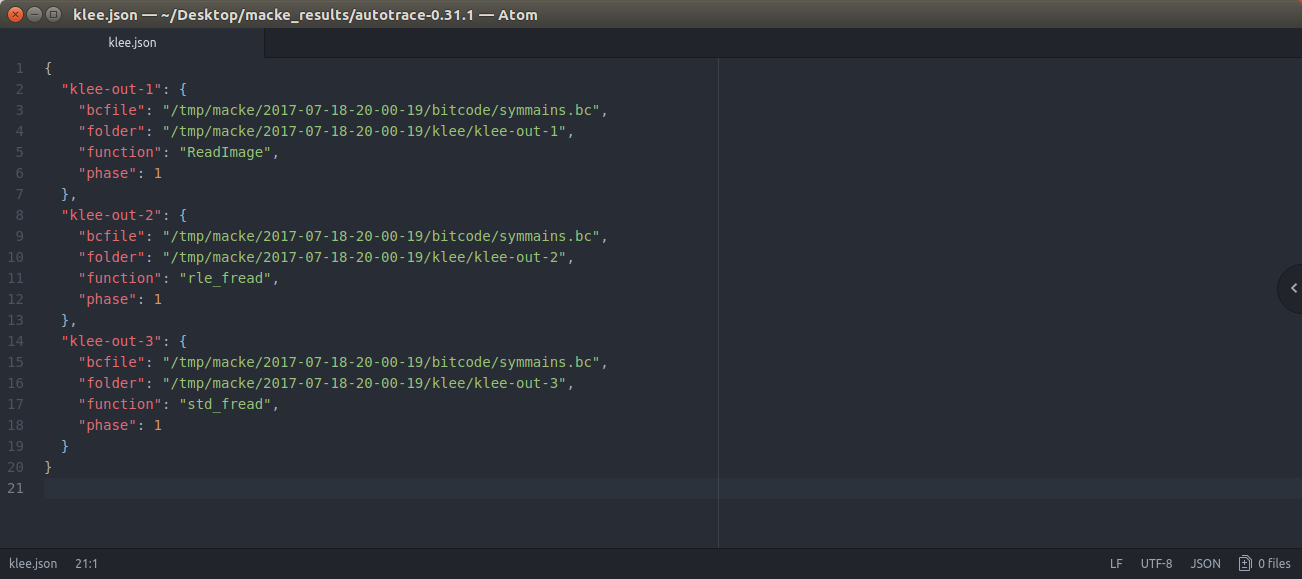
\includegraphics[width=1.0\textwidth]{macke_result}
\end{figure}

The results confirmed that compositional symbolic execution has a high source code coverage, as well as how reliable these findings were.

\subsection{Analisis of the vulnerabilities found}

The results gotten from MACKE were nothing short of outstanding. As seen on figure 3.6, MACKE found 3 vulnerabilities, two of which were documented on the NVD database, as shown in Figure 3.7 and 3.8:

\begin{figure}[!htb]
	\caption{NVD documented error for ReadImage}
	\centering
	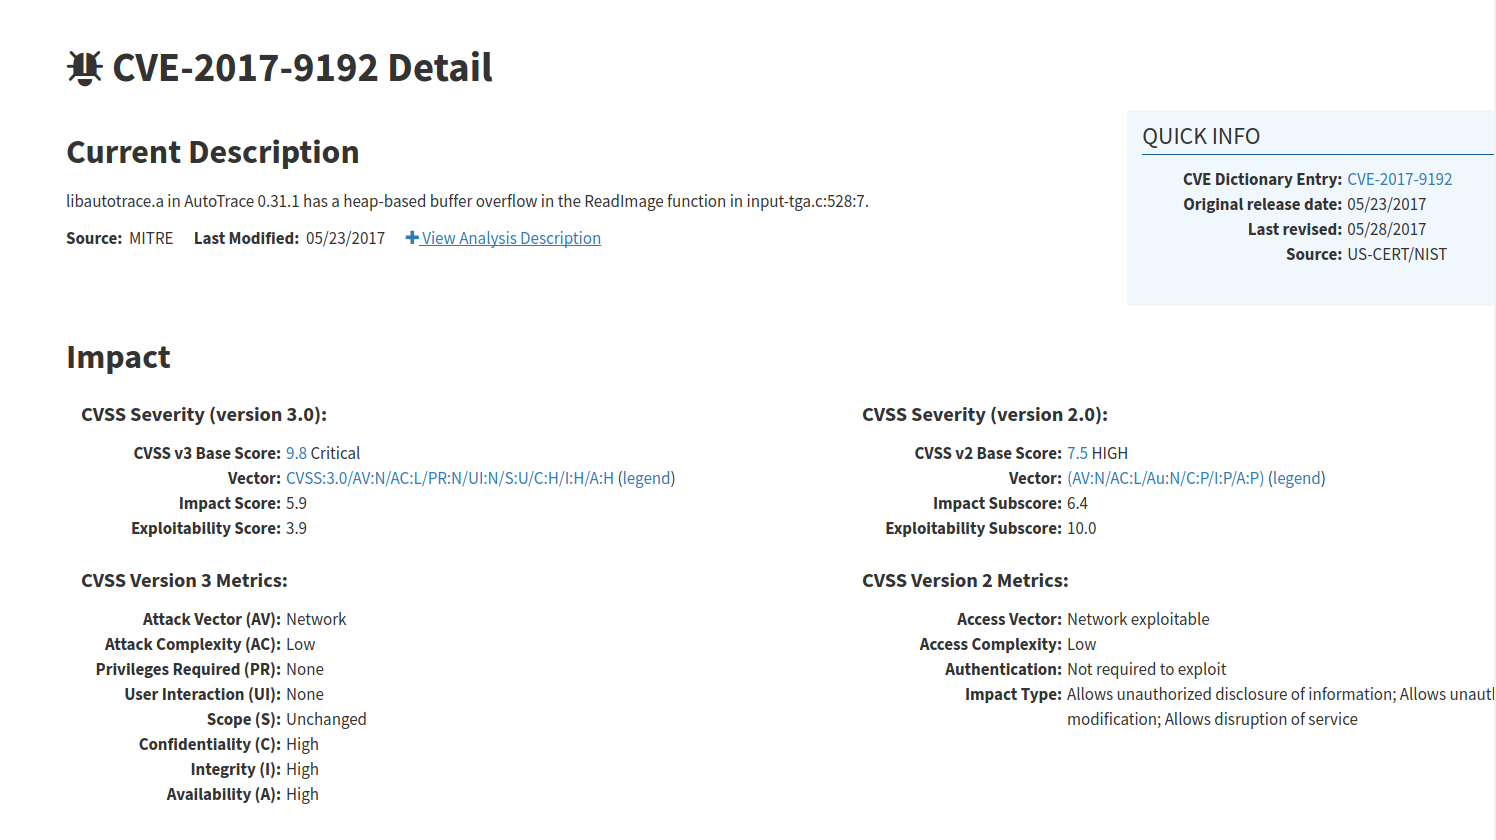
\includegraphics[width=1.0\textwidth]{readImage_error}
\end{figure}

\begin{figure}[!htb]
	\caption{NVD documented error for rlefread}
	\centering
	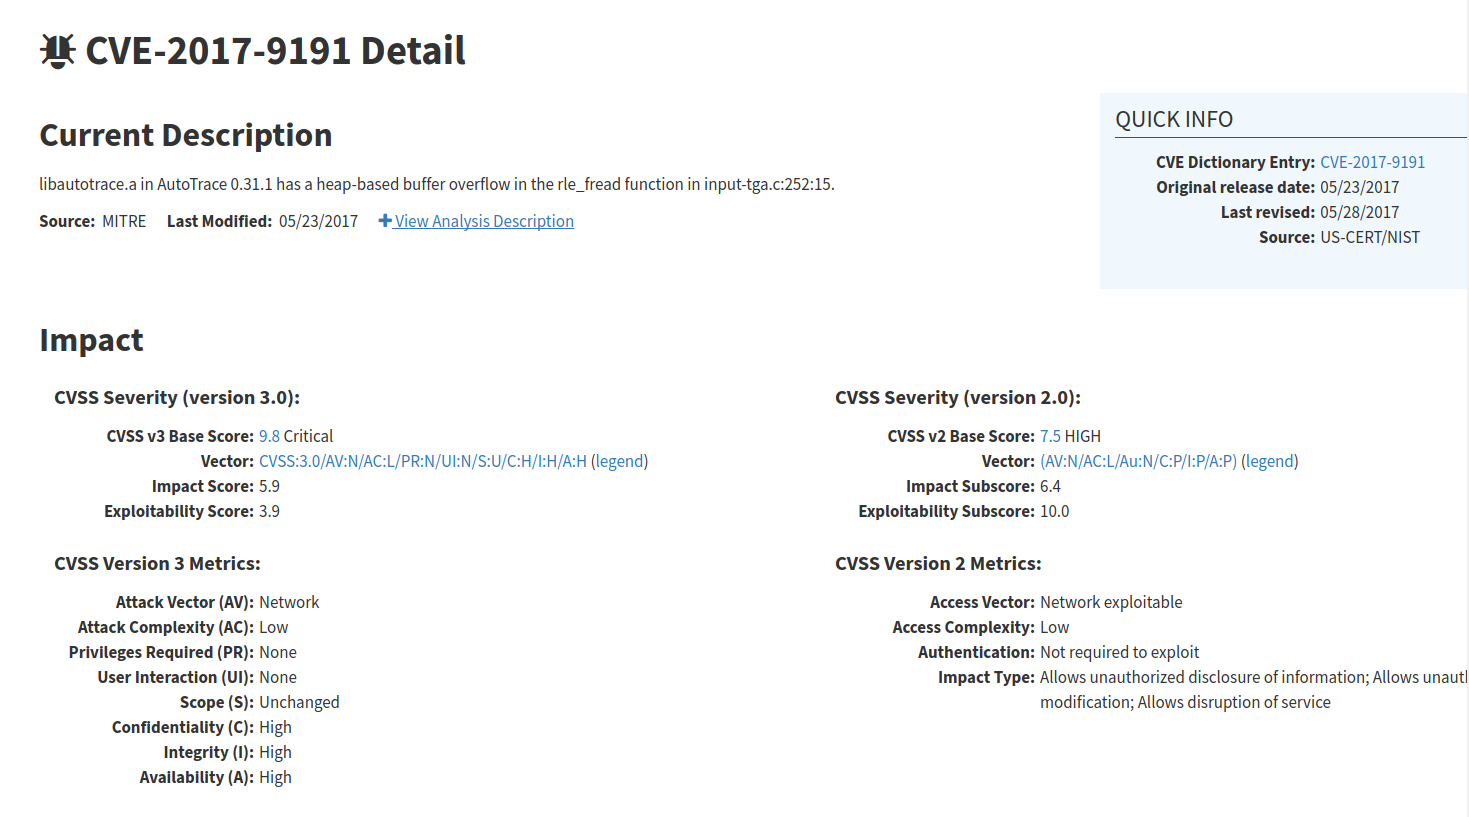
\includegraphics[width=1.0\textwidth]{rleFread_error}
\end{figure}

As shown in the aforementioned figures, MACKE found a 100\% of the vulnerabilities documented, on top of one more, which will come in handy in the future. 

What we can do now by doing the analisis of this documented vulnerabilities is the following:

\begin{enumerate}
	\item Store the CVSS3 for the functions found in the database AND in the MACKE results
	\item Calculate the node attributes of all nodes (both where vulnerabilities have been found, and where none have been found)
	\item Do these two previous steps for all programs mentioned previously
	\item Analyze the correlation and covariance between the node attributes, and their CVSS3 scores.
\end{enumerate} 

After these steps are done, we would be in good standing to develop a learning algorithm that can predict the CVSS3 scores based on the node attributes.

\subsection{Calculating node attributes}

A very crucial part of our thesis is the extraction of some node attributes on a per node basis, and to do this, as mentioned previously, we need to generate a callgraph of each program. In order to do this we require "llvm-opt" which is part of the LLVM \parencite{llvm} set of tools.

To extract the node attributes we need to run the following command:

\begin{lstlisting}[language=bash]
$ opt -analyze -dot-callgraph BITCODE_FILE.bc
\end{lstlisting}

This command will generate a call graph in .dot file format, which is a graph description language \parencite{dot} which is a static callgraph, which means it will display all relationships found in the code, yet not only the ones shown during runtime, and precisely what we need to analyze the graph features of it.

The callgraph for AutoTrace 0.31.1 looks as follows:

\begin{figure}[!htb]
	\caption{AutoTrace 0.31.1 callgraph with redundant edges}
	\centering
	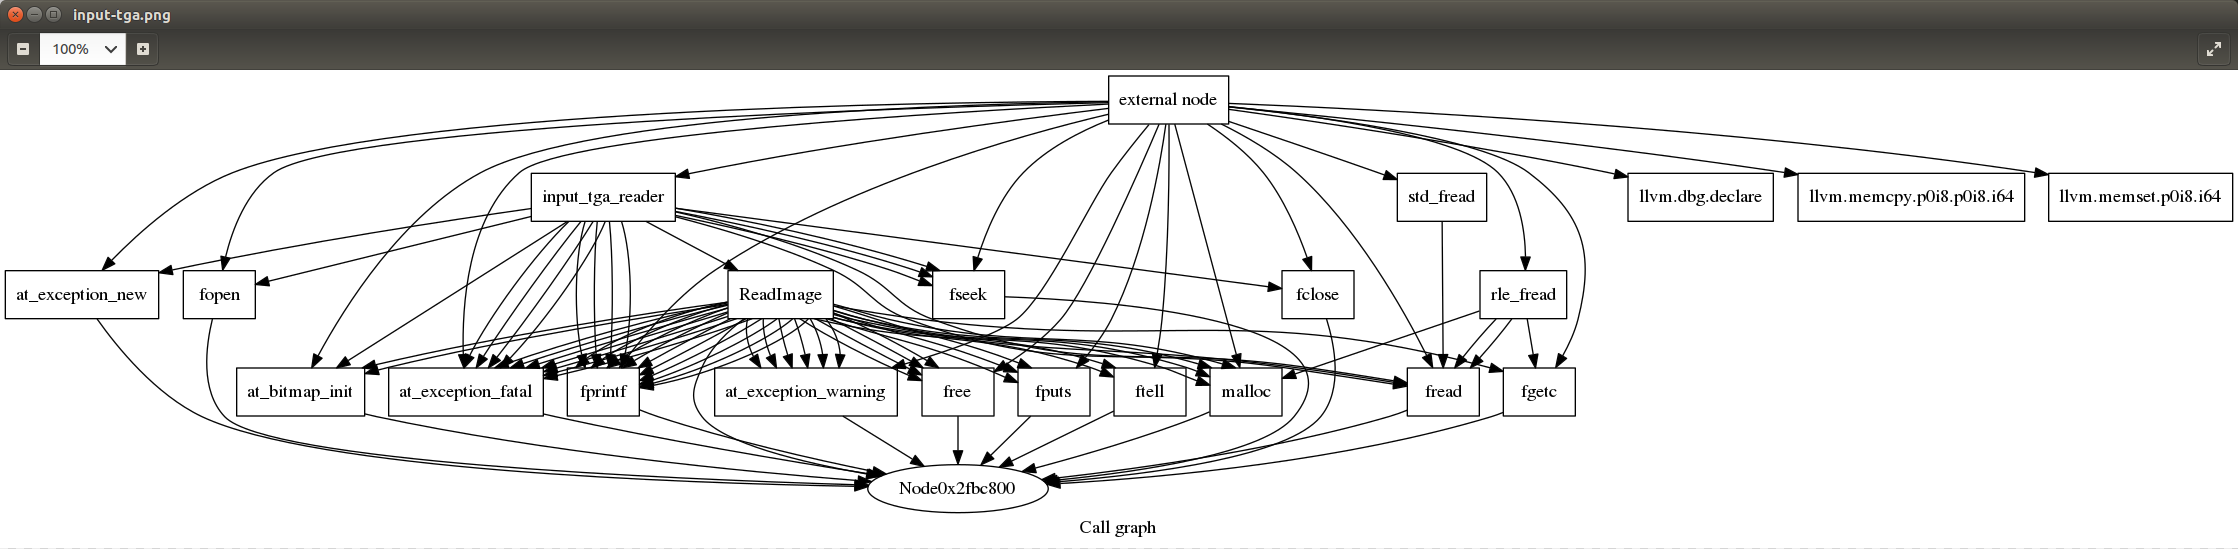
\includegraphics[width=1.0\textwidth]{callgraph_autotrace_notfixed}
\end{figure}

At first glance it is easy to see one of the underlying problems of static call graphs, which is having several edges that have the same source and target. The reason of this issue appearing in static call graphs is that, if for instance function $a$ calls function $b$ in different ocations depending on its received parameters (e.g a branch of the function), all of these calls will be extracted and none will be disregarded.This not only would render the analysis of the graph useless, since all the values would be completely off.

Seeing this we set out to clean the graph, and remove all redundant edges. To do this we used the .dot file as our input in our node attributes program, which has been developed using Python as the programming language. A snippet of the part where we remove this redundancies looks as follows:

\begin{lstlisting}[language=python]
def generate_tree(entry_node, root, visited=None):
	if visited is None:
		visited = set()
	for link in data["links"]:
		if entry_node in link["source"]:
			key = hash(entry_node + link["source"] + link["target"])
			if key not in visited:
			visited.add(key)
			name = find_label(link["target"])
			new_node = Node(name, parent=root)
			generate_tree(link["target"], new_node, visited)
	return root
\end{lstlisting}

By doing this we did two things: we were able to create a tree representation of the callgraph as a structure in Python for easy manipulation and analysis, as well as the complete removal of all the redundant edges. The resulting callgraph is shown in Figure 3.10.

\begin{figure}[!htb]
	\caption{AutoTrace 0.31.1 callgraph without redundant edges}
	\centering
	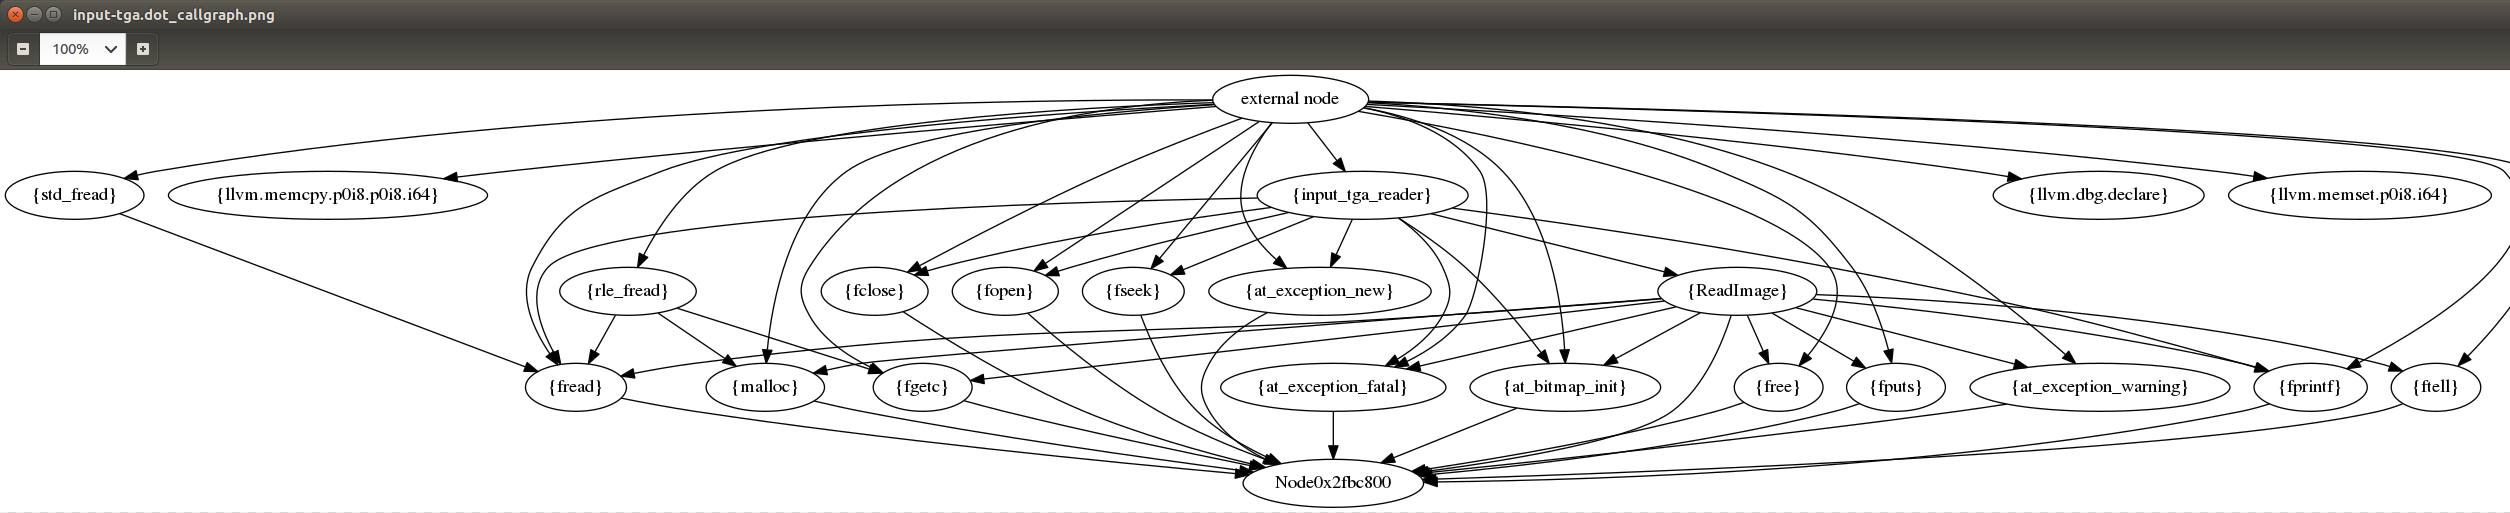
\includegraphics[width=1.0\textwidth]{callgraph_autotrace_fixed}
\end{figure}

\begin{figure}[!htb]
	\caption{AutoTrace 0.31.1 node attributes JSON file}
	\centering
	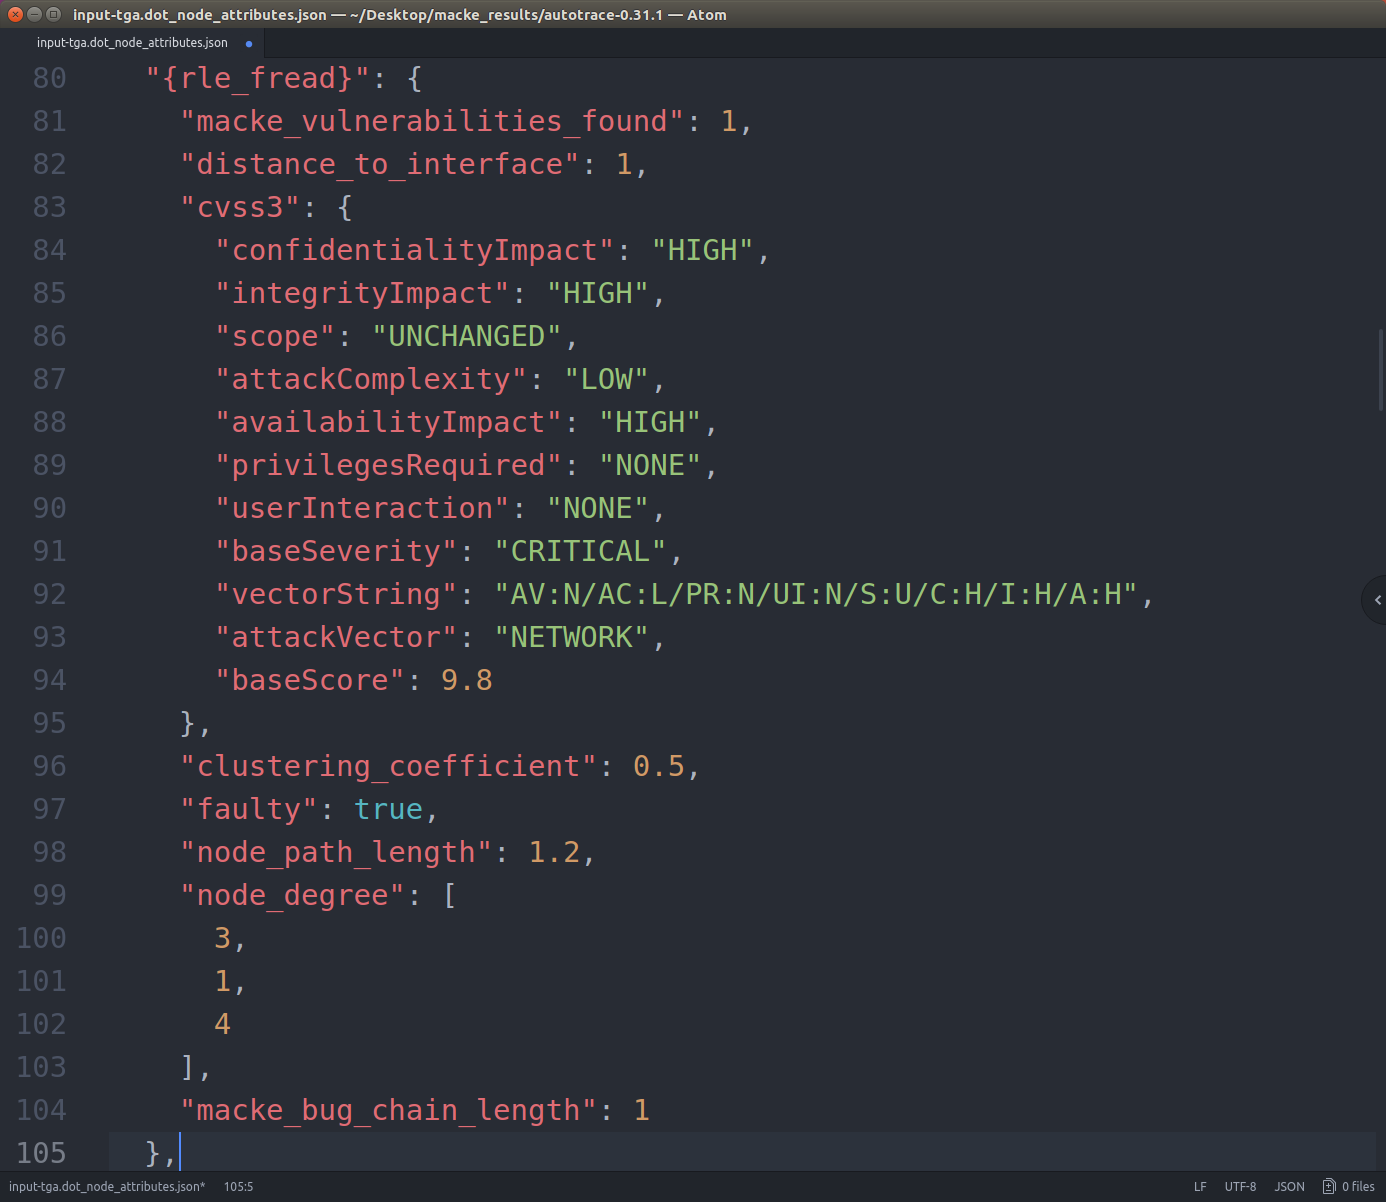
\includegraphics[width=1.0\textwidth]{node_attributes_example}
\end{figure}

With this in callgraph we would be able to analyze as needed, knowing that the graph attributes would be accurate.

The next step taken was the extraction of each node attributes for each node. To do this we used the tree structure mentioned previously. We were able to extract all node attributes successfuly by analyzing the tree and using the logic described in 3.1.5 without problems after solving the aforementioned problem.The complete source code developed throughout this thesis can be found at \parencite{ricardo} .


The node attributes resulting file encoded in JSON as shown in Figure 3.11 .

\subsection{Correlation found}


Right from the beginning, we set out to develop a way to test the correlation and covariance found between the node attributes, and the CVSS3 scores found in the NVD database. In order to do so, we developed a function, with the help of the library numpy \parencite{numpy} that would allow us to do so. The part of the entire codebase developed for this can be found at \parencite{ricardo} .

The results found are shown in Figure 3.12

\begin{figure}[!htb]
	\caption{Correlation found of node attributes to CVSS3 scores}
	\centering
	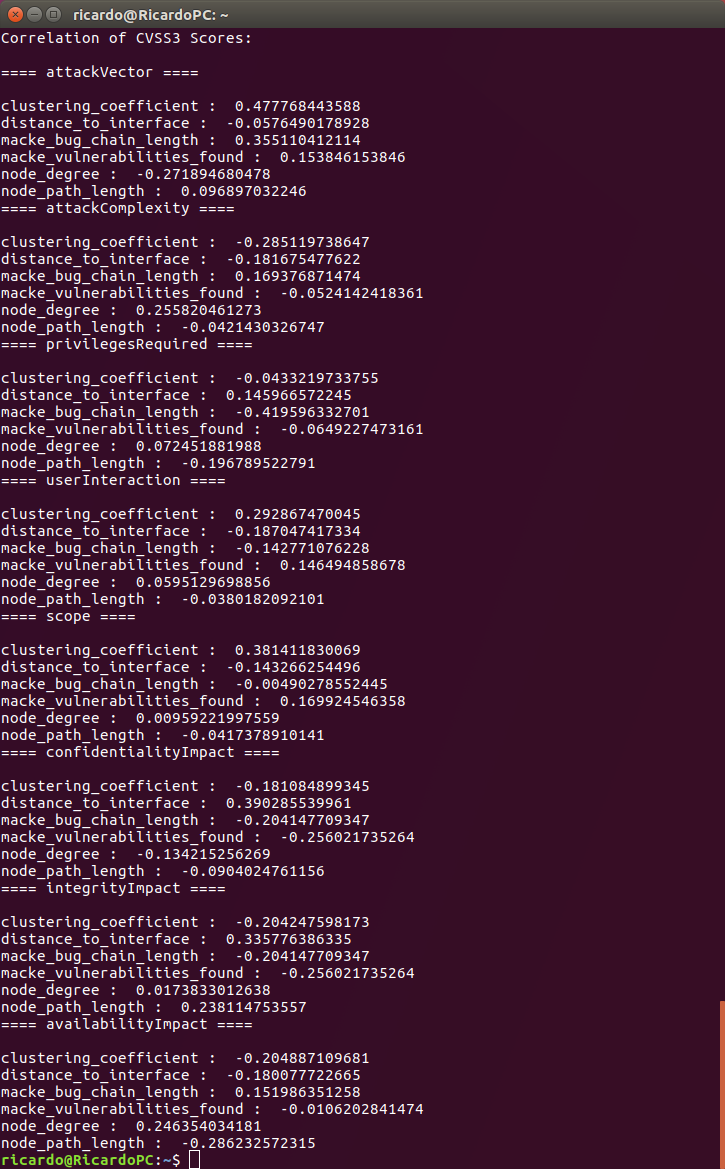
\includegraphics[width=1.0\textwidth]{correlation}
\end{figure}

Out of these results we were able to tell that the correlation for some node attributes was really small, which allowed us to have an idea how important, or irrelevant some node attributes were regarding some CVSS3 base scores. Furthermore, we also thought that while the results were not so encouraging, we needed to use this data for learning, and see how accurate it could actually be.

\subsection{Learning CVSS base score values from node attributes}

Once we had a ll of the previous parts developed, we set out to develop a learning function tha would:

\begin{itemize}
	\item Have its $X$, or contstant value be the node attributes.
	\item Have a different $y$ value for each CVSS3 base attribute.
\end{itemize}

Therefore, we would be able to generate a model that based on the node attributes, and all of the CVSS3 scores at hand, could predict new base scores solely based on node attributes given to it.

In order to do this we used one of the biggest machine learning libraries for Python, called scikit \parencite{scikit}, which allowed us to use several different machine learning algorithms to find whether or not some would fit our needs. The results will be discussed in detail in Chapter 4.
\subsection{Framework implementation}
test